\section{Astrophysical Models}
\label{sec:models}

%==============================================================================
\subsection{Basic Assumptions}
\label{sec:basic}

\cfg{why do we have error bars, if these are basically the mean
of the ucla and mpe values?}

In this paper, we assume the mass of and distance to \sgra are
\begin{align}
  \mbh &= (4.14  \pm 0.014) \times 10^6 \msun, \label{eq:mass} \\
  D    &= (8.127 \pm 0.023) \kpc,              \label{eq:dist}
\end{align}
which are approximately the mean of values reported by \citet{2019Sci...365..664D} and \citet{2019A&A...625L..10G}.

Throughout the paper we also assume that \sgra is a black hole and described by a Kerr spacetime.
The black hole dimensionless spin, $\abh \equiv Jc/G\mbh^2$, is a free parameter with $-1 < \abh < 1$.
Here, $J$, $G$, and $c$ are the black hole angular momentum, gravitational constant, and speed of light, respectively.
Following \citetalias{M87PaperV},
$\abh > 0$ indicates the angular momentum of the accretion flow and black hole are parallel (the accretion flow is ``prograde'') and
$\abh < 0$ indicates the angular momentum of the accretion flow and black hole are antiparallel (``retrograde'').

Using the above mass and distance, the implied
characteristic length $r_\mathrm{g}         \equiv G\mbh/ c^2    \simeq 6.1\times10^{11}\cm$,
characteristic time   $t_\mathrm{g}         \equiv G\mbh/ c^3    \simeq 20.5\sec$, and
angular scale         $\vartheta_\mathrm{g} \equiv G\mbh/(c^2 D) \simeq 5.03\uas$.
The expected diameter of the black hole shadow is $2\sqrt{27} G\mbh/(c^2 D) = (52.2 \pm 2.08)\uas$,
where errorbars enclose uncertainty in the black hole spin and viewing angle \citep[see, e.g.,][]{2013ApJ...777...13C, 2020ApJ...896....7M}.

If the emitting plasma is ionized hydrogen (electron-proton plasma), then the Eddington luminosity is
$L_\mathrm{Edd} = 4\pi G\mbh c m_p/\sigma_{T} = 5.2 \times 10^{44}\ergsps$.
The corresponding Eddington accretion rate is
$\dot\mbh_\mathrm{Edd} \equiv L_\mathrm{Edd}/(0.1 c^2) = 5.8 \times 10^{24} \gm \sec^{-1} = 0.09 \msun \yr^{-1}$,
where nominal efficiency is 10\% and the Eddington ratio:
$L_\mathrm{bol}/L_\mathrm{Edd} = 1.9 \times 10^{-10} (L_\mathrm{bol} /10^{35})$,
where $L_\mathrm{bol}$ is in unit of $\ergsps$.
In a quiescent, non-flaring state, the bolometric luminosity of \sgra is $L_\mathrm{bol} \sim 10^{35}\erg\sec^{-1}$, resulting in an extremely small Eddington ratio.
In what follows, we will assume that the radiative cooling of plasma around the black hole can be neglected and that model emission can be calculated as post-processing.

%==============================================================================
\subsection{Estimate from One-Zone Model}

The development of complex models is guided by simple estimates.
Following \citetalias{M87PaperV}, we first consider an one-zone model for \sgra.
These results follow one-zone models developed in the literature over many decades (refs).

Our one-zone model is a uniform plasma sphere of radius $r = 5\rg$ with uniform magnetic field oriented at $\pi/3$ to the line-of-sight.
The magnetic field is given by $n_i k T_i + n_e k T_e = \beta B^2/(8\pi)$, where $T_i$ denots ion temperature, $T_e$ denotes electron temperature, $\beta=1$, and $T_i = 3 T_e$.
We also assume $\Theta_e \equiv  k T_e / m_e c^2 = 10$.

Using the thermal emissivity for synchrotron radiation $j_\nu$ \citep[e.g.,][]{2011ApJ...737...21L} and assuming optically thin emission, the flux density is given by $F_\nu = (4/3)\pi r^3 j_\nu D^{-2} 10^{23}\,\mathrm{Jy}$.  Setting $F_\nu = 2.4\,\mathrm{Jy}$ (the average measured by ALMA during the 2017 campaign) yields a nonlinear equation for $n_e$ with solution
\begin{align}
  n_e &\simeq 1.1\times10^6\cm^{-3},\\
  B   &\simeq 30\,\mathrm{G}.
  \label{eq:onezone}
\end{align}
(the synchrotron optical depth $\tau_\mathrm{sync} = r j_\nu/B_\nu \simeq 0.4$, so the optically thin approximation is marginal).
These values are consistent with $n_e$ and $B$ of a similar one-zone model fitted to archival \sgra millimeter spectrum as reported in \citet{2019ApJ...881L...2B}.
%MM: fit of similar one zone model to Terahertz spectrum from ALMA infers ne=2-5x10^6 cm^-3, B=10-50 Gauss, T_e=1-3x10^11 K => Thetae=16-50
% CFG: I've placed a mathematica script implementing the one zone model in eht.astro.illinois.edu://bd4/eht/paperV/OneZoneThin.ma

The one-zone model has optical depth to Compton scattering $\tau_e \sim \sigma_T n_e r \simeq 2\times10^{-5}$, and thus a small Compton parameter: $y = 16 \Theta_e^2 \max(\tau_e,\tau_e^2) \simeq 3\times10^{-2}$.
Synchrotron cooling therefore dominates Compton cooling.

The synchrotron cooling timescale is $t_\mathrm{cool} \equiv u/\Lambda$ where $u_e = 3 n_e k T_e$ is the electron internal energy and $\Lambda \simeq 5.4 B^2 e^4 n_e \Theta_e^2 /(c^3 m_e^2)$ is the synchrotron cooling rate from thermal population of electrons with $\Theta_e \gtrsim 1$ (for details see Appendix~A in \citealt{2011ApJ...735....9M}; finite optical depth reduces $\Lambda$).
The cooling time in the one-zone model is therefore $t_\mathrm{cool}=2.3 \times 10^4\sec \simeq 1.1 \times 10^3 \tg$ which is longer than the characteristic inflow time.
Cooling can therefore be neglected in the numerical models \citep[e.g.,][]{2012MNRAS.426.1928D}.\footnote{Notice that if \sgra is fed by stellar winds then the inflowing plasma may be mainly helium \citep{2019MNRAS.482L.123R}; this changes the one-zone model only slightly.  Helium accretion is discussed  in Appendix~\ref{app:variability}.}

The one-zone model implies that the accretion flow is at high temperature and low density and is therefore collisionless, in the sense that the mean free path to Coulomb scattering is large compared to $\rg$.
At $\Theta_e \sim 1$, for example, the Coulomb scattering cross section is comparable to the Thomson cross section, and the mean free path therefore $\sim \tau_e^{-1} \rg$.
The electron-ion Coulomb scattering timescale is also long, and the electrons and ions are therefore poorly coupled.
This motivates consideration of
\emph{i})~a two-temperature model for the plasma where electrons are cooler than the ions \citep{1976ApJ...204..187S,1977ApJ...214..840I, 1982Natur.295...17R} and
\emph{ii})~nonthermal (unrelaxed) electron distribution functions.
As discussed in \citet{2000ApJ...541..234O}, \citet{2009ApJ...701..521C}, and \citet{2014A&A...570A...7M} \citep[see also more recent work by][]{2018A&A...612A..34D,2021arXiv211102518F, 2021NatAs.tmp..218C, 2021arXiv211203933E}, both effects may change the predicted properties of \sgra.
%\br{my only remaining comment is that I think that the sentence ``As demonstrated in \citet{2000ApJ...541..234O} and \citet{2014A&A...570A...7M} (see also more recent work by \citealt{2018A&A...612A..34D} and references therein) both effects may change the predicted properties of \sgra.'' should be cut, or extended with non-EHT refs on how other groups actually probe those collisionless effects dynamically}
\ckc{In principle, we could numerically check all of the assumptions in the one zone model for consistency.  Probably leave until after PC submission.}
\monika{i think that the purpose of this section is to make a rough estimates on the back of the envelope so that everyone can repeat them, numerical work is always more difficult to repeat}
\ckc{Yes but these also usually physical interesting quantities.  At least we should compute the values that paper~I wants.}

%==============================================================================
\subsection{Numerical Models of the Inner Accretion Flows}

\begin{deluxetable*}{cccccccc}
  \tabletypesize{\footnotesize}
  \renewcommand{\arraystretch}{1.1}
  \tablehead{                     &
    \colhead{Spacetime}           &
    \multicolumn{2}{c}{Fluid}     &
    \multicolumn{3}{c}{Numerical} &
    \colhead{Note} \\
    \colhead{Setup/Code}                  &
    \colhead{$\abh$}                     &
    \colhead{Mode}                       &
    \colhead{$\Gamma_\mathrm{ad}$}       &
    \colhead{\!\!\!\!\!\!$t_\mathrm{final}$ [$\rg$]} &
    \colhead{Size [$\rg$]\!\!\!\!\!\!}               &
    \colhead{Resolution}                 &
    \colhead{Reference}
  }
  \startdata
  \begin{tabular}{@{}c@{}} standard / \\ \kharma \end{tabular} & 0,$\pm1/2$,$\pm15/16$                 & MAD/SANE     & $4/3$      & 30,000  & 1000     & [288x128x128]     & \!\!\!\!\!\!\!\!\!
   \begin{tabular}{@{}c@{}c@{}} This work\\\citet{Wong_2022} \\ \citet{Dhruv_2022}\end{tabular}\\
%  \citet{Wong_2022, Dhruv_2022} \\
  \begin{tabular}{@{}c@{}} standard / \\ \bhac \end{tabular}   & 0,$\pm1/2$,$\pm15/16$                 & MAD/SANE     & $4/3$      & 30,000  & 3333     & [512x192x192]     & This work \\
  \begin{tabular}{@{}c@{}} standard / \\ \hamr \end{tabular}   & 0,$\pm1/2$,$\pm15/16$                 & MAD/SANE     & $13/9,5/3$ & 35,000  & 1000/200 & [348/240×192×192] & This work \\
  \begin{tabular}{@{}c@{}} standard / \\ \koral \end{tabular}  & \!\!\!\!\!\!\!\!\!
  \begin{tabular}{@{}c@{}c@{}}   0,$\pm0.3$,$\pm0.5$\\$\pm0.7$,$\pm0.9$ \end{tabular}
  \!\!\!\!\!\!\!\!\! & MAD          & $13/9$     & 101,000 & 100,000  & [288x192x144]     & \citet{2021arXiv210812380N} \\
  \begin{tabular}{@{}c@{}} tilted / \\ \hamr \end{tabular}     & $15/16$     & IN-SANE      & 5/3        & 105,000 & 100,000  & [448x144x240]     & \begin{tabular}{@{}c@{}} \citet{Liska2018} \\ \citet{Chatterjee2020}\end{tabular} \\
  \begin{tabular}{@{}c@{}} wind-fed / \\ \athenapp \end{tabular} & 0           & MAD$\times2$ & 5/3        & 20,000  & 2,400    & [356x128x128]     & \citet{2020ApJ...896L...6R}
  \enddata
  %\tablenotetext{$*$}{Non-standard model.}
  \caption{Summary of GRMHD simulations in the EHT \sgra GRMHD model library.
    The first four entries are standard \sgra simulations.
    The last two entries are the tilted accretion model and two realizations of the Wind Accretion models which differ in stellar wind magnetization.}
  \label{tab:GRMHDmodels}
\end{deluxetable*}

The one-zone model is too simple for comparison with the rich set of observations available for \sgra.
Going beyond the one zone model, analytic spherical accretion models \citep[e.g.][]{2019ApJ...885L..33N, 2021arXiv211102178B} incorporate relativistic  gravity and analytic disk-like (RIAF) accretion models in the Kerr metric incorporate rotation and departures from spherical symmetry \citep[e.g.][]{2009ApJ...697...45B, 2009ApJ...706..960H,2018ApJ...863..148P} can be used for parameter surveys (see Section~\ref{sec:future}).
% I think the previous sentence says both analysis spherical and disk can be used for blab blab blab...  Minor edit to retain that meaning.
They do not, however, self-consistently capture fluctuations in the flow---that requires either a statistical model \citep{2021ApJ...906...39L} or a time-dependent numerical integration.
\ckc{May be also say they don't self-consistently capture turbulence for transport.}
Here we use numerical simulation and adopt an ideal GRMHD model for the flow \footnote{Limitations of the ideal GRMHD model are discussed in Section~\ref{sec:limits}.}, use simple parameterized models to assign an electron distribution function, and solve the radiative transfer equation along geodesics to produce synthetic observations.

%------------------------------------------------------------------------------
\subsubsection{Plasma Flow Model}

We model the plasma flow around \sgra using ideal, non-radiative GRMHD.
The gravitational field is given by the Kerr metric, with mass given by Equation~(\ref{eq:mass}) and with black hole spin $\abh$ as a free parameter \citep[see e.g.,][]{2003ApJ...589..444G, 2005ApJ...635..723A, 2007A&A...473...11D}.

We integrate the GRMHD equations in three spatial dimensions using multiple algorithms:
\kharma   \citep{2021JOSS....6.3336P},
\bhac     \citep{2017ComAC...4....1P},
\hamr     \citep{Liska2018},
\koral    \citep{2013MNRAS.429.3533S}, and
\athenapp \citep{2016ApJS..225...22W};
see \citet{2019ApJS..243...26P} and \citet{Olivares_et_al} for comparisons of GRMHD codes.
All simulations assume a constant adiabatic index $\Gamma_\mathrm{ad}$.

The \emph{standard} initial conditions for the GRMHD integrations are a hydrodynamic, constant-angular-momentum equilibrium, the Fishbone-Moncrief torus \citep{1976ApJ...207..962F}
%\aco{\citep[see also][]{2002MNRAS.334..383F}} \monika{why do we need to have this second citation? is that essential?} \br{I thought Font shows another hydro torus equilibrium in this paper? We don't use that one, so I would not cite that paper} \ckc{all modelers: do any of you use the Font initial condition?  If not I will comment out this reference.}\aco{There are two independent hydro solutions, we have both of them. With same initial condition for magnetic field on top of hydro-solution}\br{is there a reason for using different initial conditions? I tried both FD and FM torus myself and the FD torus evolution is somewhat different. It would be better to start from the same IC to compare late states of the models to images. Which models exactly do use the (different) initial conditions of the Font-Daigne torus? I thought in paper V for M87 we used only the FM torus. Then the first sentence in this paragraph above is also wrong, because we are not using the FM torus exclusively.}\monika{exactly which model in the library starts from FD torus? please answer before midnight.} % \aco{Yes, I think is essential to cite, is true that we not using FD but we also have it in BHAC. Please be free to remove it. But definitively don't have same initial condition in all GRMHD codes.}
% /monika{11dec: we dont want to elaborate on details like that here, this section is intended to describe only common features of all simulations, other details can be described in section 4.]
in a prograde ($\abh > 0$) or retrograde ($\abh < 0$) orbit.
In all models except the \hamr-Tilted models the torus orbital angular momentum is either parallel or antiparallel to the black hole spin. The torus is parameterized by an inner radius $R_{\rm in}$, typically $12\rg$, and the pressure maximum radius $R_\mathrm{max}$, typically $24\rg$.
%\aco{We should specify the torus size? or should we refer to the reader to SANE and MAD code comparison. We have different initial data between codes, not only in the size but also in adiabatic index in the equation of state.}
%\aco{ with magnetization $\beta \equiv p_{\rm gas}/p_{\rm mag} =100$}
%\monika{11dec: we dont want to elaborate on details like that here, this section is intended to describe only common features of all simulations, other details can be described in section 4, incase there are differences in the results that may be due to initial conditions.}
The torus is seeded with a weak, poloidal magnetic field.

The torus initial conditions are motivated by the notion that the near-horizon flow, where most of the emission is generated \citep{M87PaperV} relaxes to a statistically steady state that is nearly independent of the flow at larger radius.  This notion is challenged in the stellar wind-fed models of \cite{2020ApJ...896L...6R}, which are included in our study.

All simulations are run in horizon penetrating Kerr-Schild coordinates, which are regular on the horizon.
Most are run in a variant of spherical polar coordinates.
The \emph{standard} boundary conditions are outflow at the inner boundary, located inside the event horizon, outflow at the outer boundary, located at $r \gtrsim 1000 \rg$, and reflecting boundary conditions at the poles.
Standard simulations are evolved to $t_\mathrm{final} = 30,000\tg$.

Once the evolution has started, a combination of instabilities including the magnetorotational instability \citep[MRI][]{1992ApJ...400..610B} drives the torus to a turbulent, fluctuating state.
Let $P_\mathrm{gas}$ be the gas pressure and $P_\mathrm{mag} \equiv B^2 / (8\pi)$ be the magnetic pressure, the standard accretion flow models can be divided by latitude into three zones:
\emph{i})~equatorial inflow,
\emph{ii})~a mid-latitude disk wind/corona with  $\beta  \equiv P_\mathrm{gas} / P_\mathrm{mag} \sim 1$, and
\emph{iii})~a polar funnel/relativistic jet with $\sigma \equiv P_\mathrm{mag} / (\rho c^2) \gtrsim 1$.

It is well established \citep[see, e.g.,][and references therein]{M87PaperV, M87PaperVIII} that the magnetic flux through the event horizon divides the outcomes into two categories: the Magnetically Arrested Disk (MAD) state \citep[e.g.,][]{1974Ap&SS..28...45B, 2003ApJ...592.1042I, 2003PASJ...55L..69N} in which the magnetic flux near the horizon saturates and significantly affects the dynamics of the flow, and the Standard and Normal Evolution (SANE) state \citep[e.g.,][]{2003ApJ...589..444G, 2003ApJ...599.1238D, 2012MNRAS.426.3241N}.
The relative importance of magnetic flux can be described by $\phi \equiv \Phi_{\mathrm{BH}} (\dot{M} r_\mathrm{g}^2 c)^{-1/2}$, where $\Phi_{\rm BH}$ is the magnetic flux interior to the black hole equator and $\dot{M}$ is the mass accretion rate through the horizon.
MAD models have $\phi \sim \phi_{\rm crit} \sim 60$.\footnote{In the Lorentz-Heaviside units commonly used in GRMHD simulations $\phi_\mathrm{crit}$ is smaller by a factor of $(4\pi)^{1/2} \simeq 3.545$.}
%\aco{Should we cite the work-in-progress by Narayan about spinup-spindown for MAD models where magnetic flux it can be written as a function of BH spin? I've verified the same tendency for BHAC.}
%\monika{not necessary, this is not established and should be first published we want to limit in prep as much as possible}
In MAD models, magnetic flux accretes onto the hole until $\phi \gtrsim \phi_\mathrm{crit}$, then magnetic flux is expelled from the hole and escapes through the inflowing plasma.
SANE models have $\phi < \phi_c$, and in most of our standard models have $\phi \sim 1$.

We also consider two \emph{non-standard} GRMHD simulations: strongly magnetized non-MAD tilted torus simulations \citep{Liska2018, Chatterjee2020} and a model in which \sgra is fed directly by winds from stars in its vicinity \citep{2020ApJ...896L...6R}.
The self-consistent wind feeding simulations result in a mode of accretion that is similar to MAD but typically has lower mean angular momentum and is less well organized.
The wind-fed models have $\abh = 0$.

The GRMHD model library is summarized in Table~\ref{tab:GRMHDmodels}.
In Figure~\ref{fig:GRMHD} we show a few examples of standard and non-standard GRMHD runs.
The models vary in numerical method and in numerical resolution. We present more information on the numerical methods and models in Appendices~\ref{app:numerical} and \ref{app:variability}.

\begin{figure*}
  \centering
  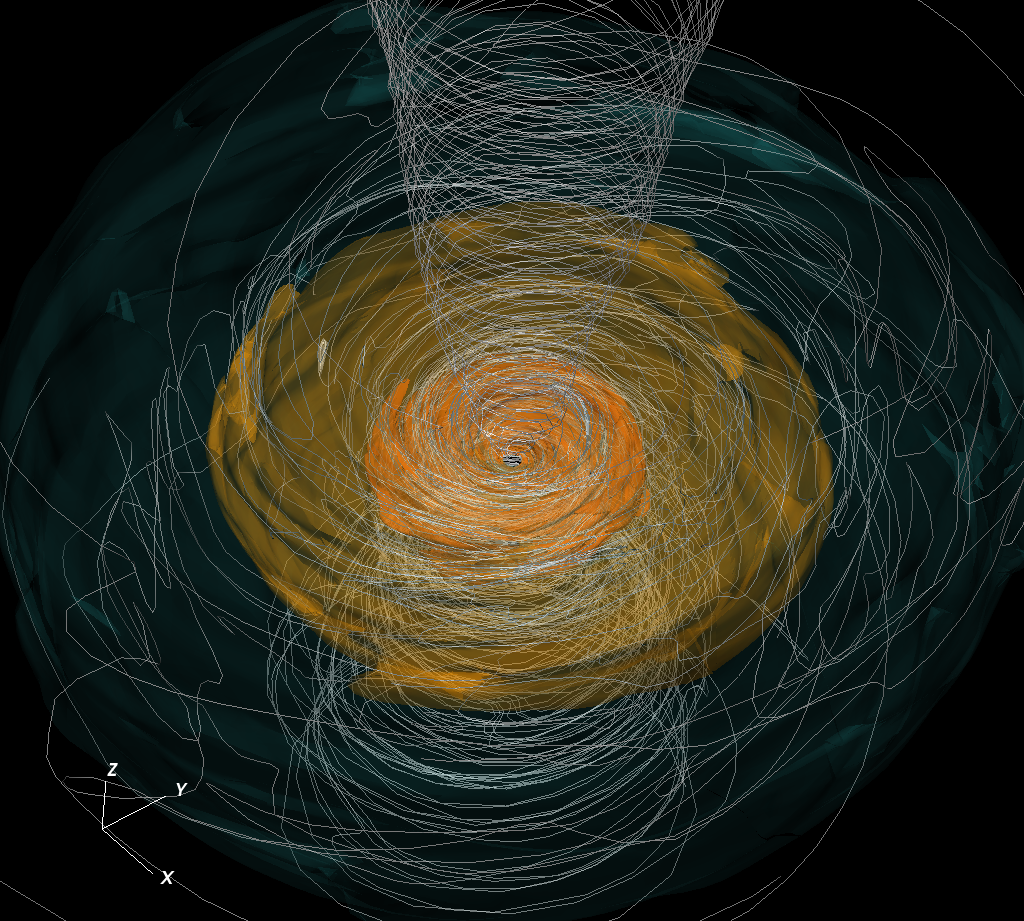
\includegraphics[width=0.4\textwidth]{figures/sane_3D.png}\hspace{1.5pt}%
  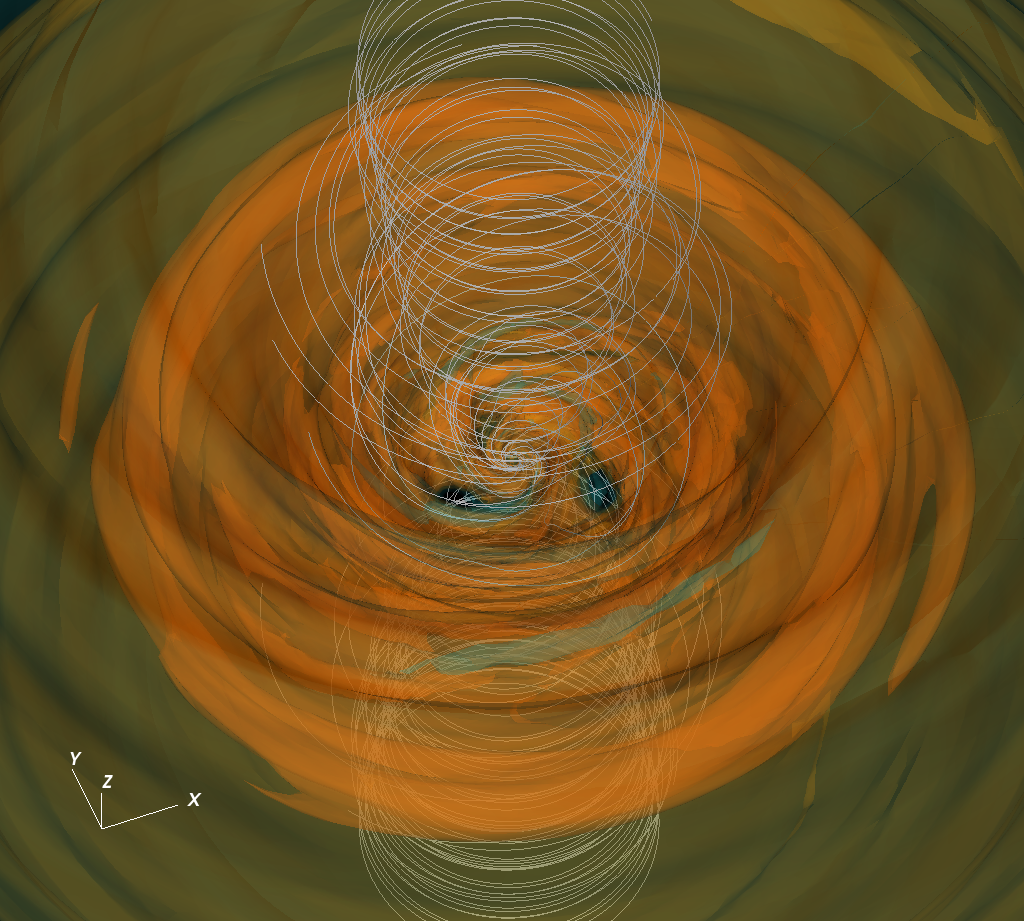
\includegraphics[width=0.4\textwidth]{figures/mad_3D_new.png}\\
  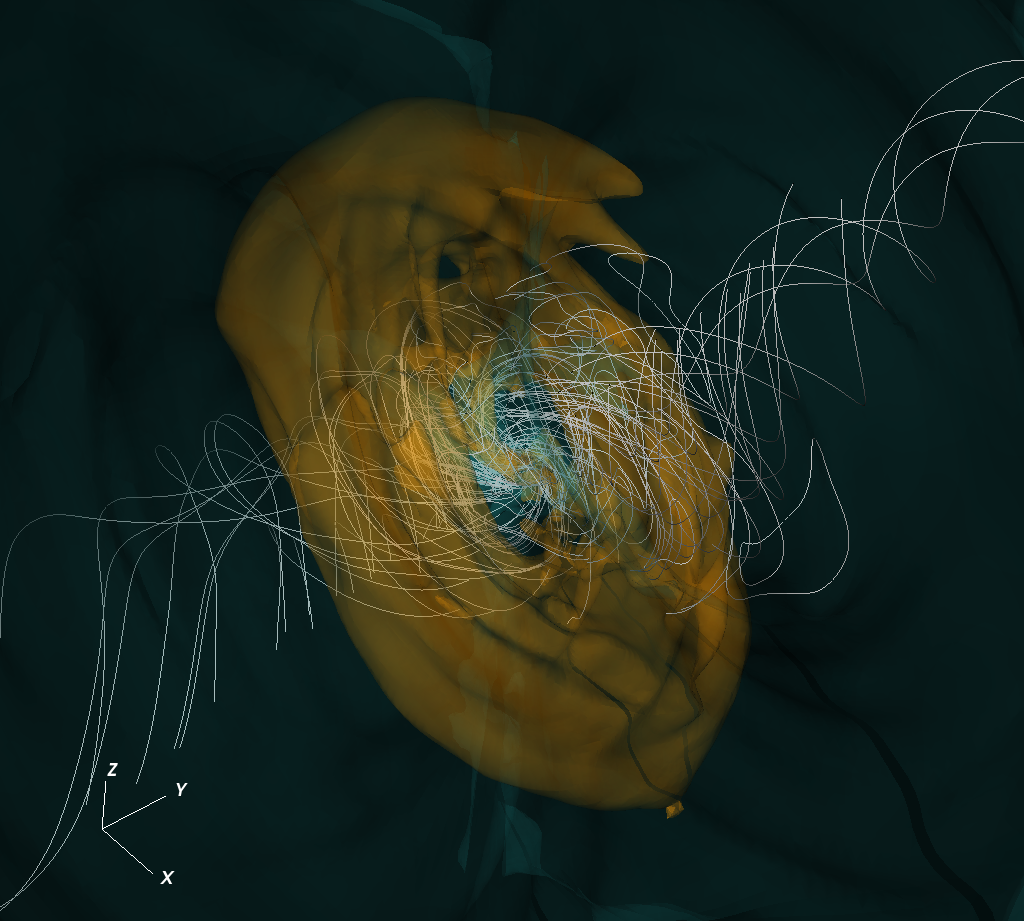
\includegraphics[width=0.4\textwidth]{figures/tilted_3D.png}\hspace{1.5pt}%
  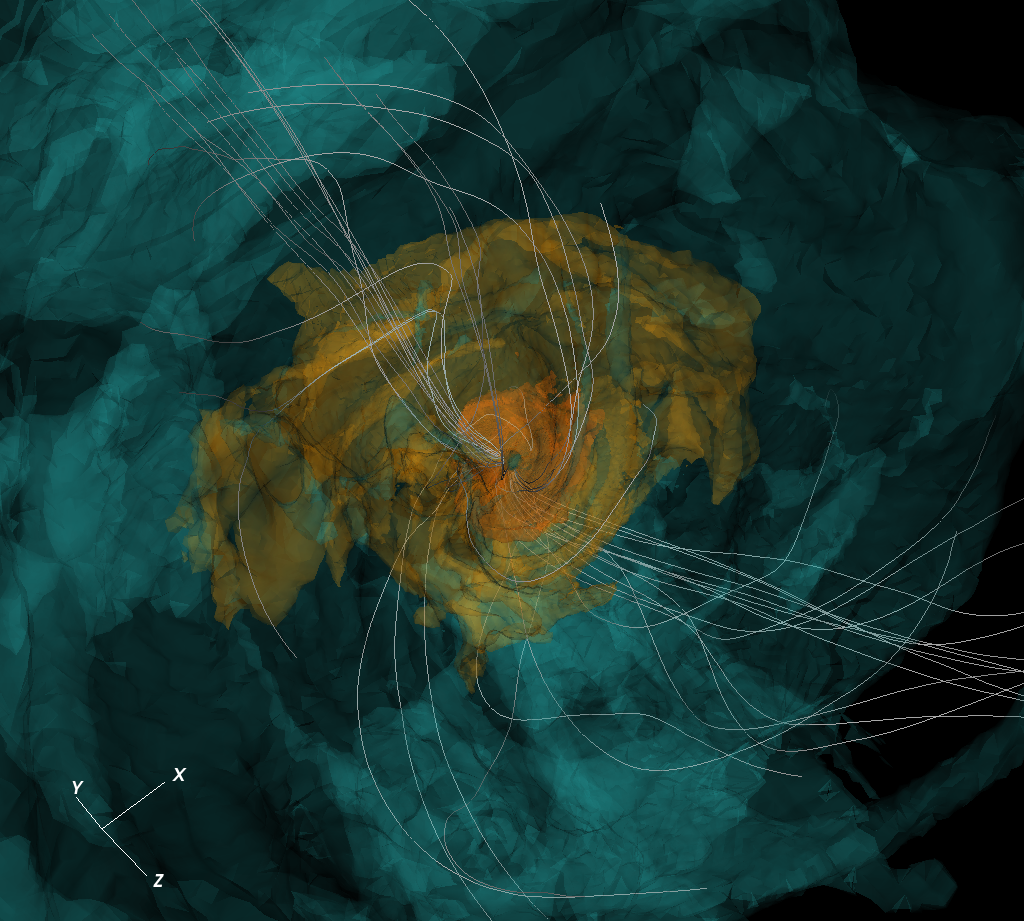
\includegraphics[width=0.4\textwidth]{figures/ressler_3D_new.png}
  \caption{3-D overview of selected GRMHD simulations of \sgra in our library.
    The color marks constant dimensionless density surfaces and lines follow magnetic field lines.
    Two top panels show standard accretion models: SANE (left panel, $\abh=+15/16$) and MAD (right panel, $\abh=0.5$).
    Two bottom panels show non-standard accretion models: tilted disk (left panel, $\abh=+15/16$ and tilt angle of $60\degree$) and Wind Accretion (right panel, $\abh=0$).
    In case of spinning black holes, the spin is aligned with z-axis.
    %\monika{plots are not final, more detailed quantitative plots of models are expected to be in the appendix.}
    %\aeb{This looks great!}
    %\gw{Presumably the MAD simulation ``only'' has field lines that thread the near-horizon region because the footpoints are distributed relative to field strength? Might be worthwhile to mention if so.}\monika{that is not the case. these images may change a bit in the near future}\gw{In that case, I definitely think we should explain how the magnetic field lines are chosen.} \aco{Monika, 3D rendering looks very nice. There are some way to choose same BH spin, view angle, limits on density and magnetic fields to see only differences in accretion models? }
    %\ckc{If these are in normal spherical polar or Cartesian, I suggest we also ask Matt Turk to try visualizing them with yt.}
    %\monika{thanks for all the suggestions, will incorporate before submission.}
  }
  \label{fig:GRMHD}
\end{figure*}

%------------------------------------------------------------------------------
\subsubsection{Radiative Transfer Model}

Synthetic observations are generated from the GRMHD model in a radiative transfer step.
The transfer step requires: %(1) CK: I prefer using i), ii), iii) in text because (1) etc are for equations.
\emph{i})~a model for the electron temperature and electron distribution function (hereafter eDF);
\emph{ii})~an assignment of a density scale to the GRMHD model;
\emph{iii})~a numerical radiative transfer step done after the GRMHD model, assuming that the plasma evolution is unaffected by radiation.

\begin{figure*}
  \centering
  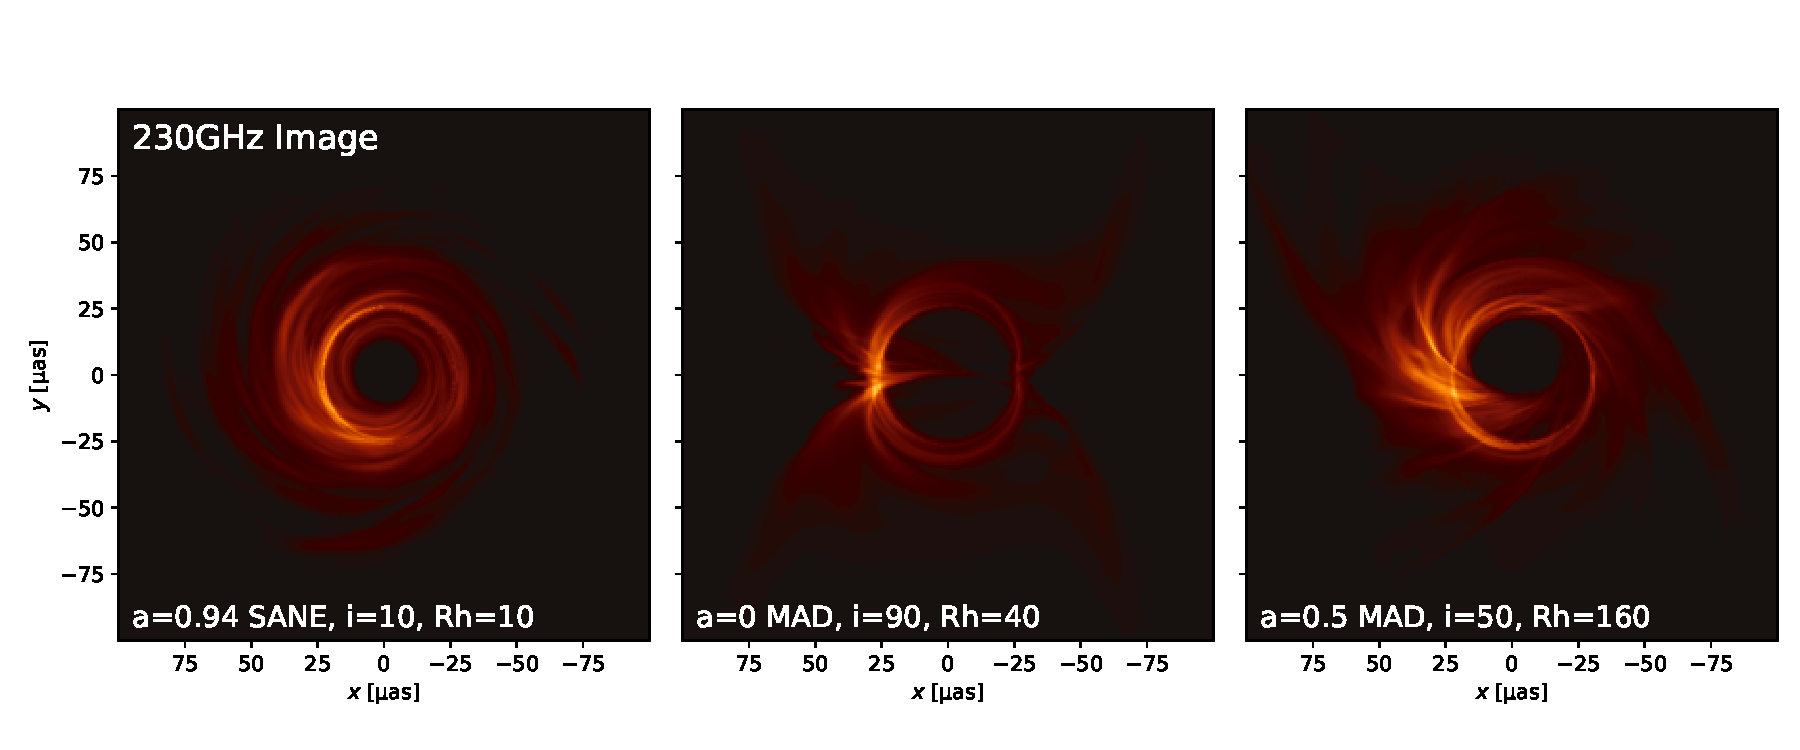
\includegraphics[width=\textwidth,trim=0 24 0 24]{figures/sample_230GHz.pdf}\\
  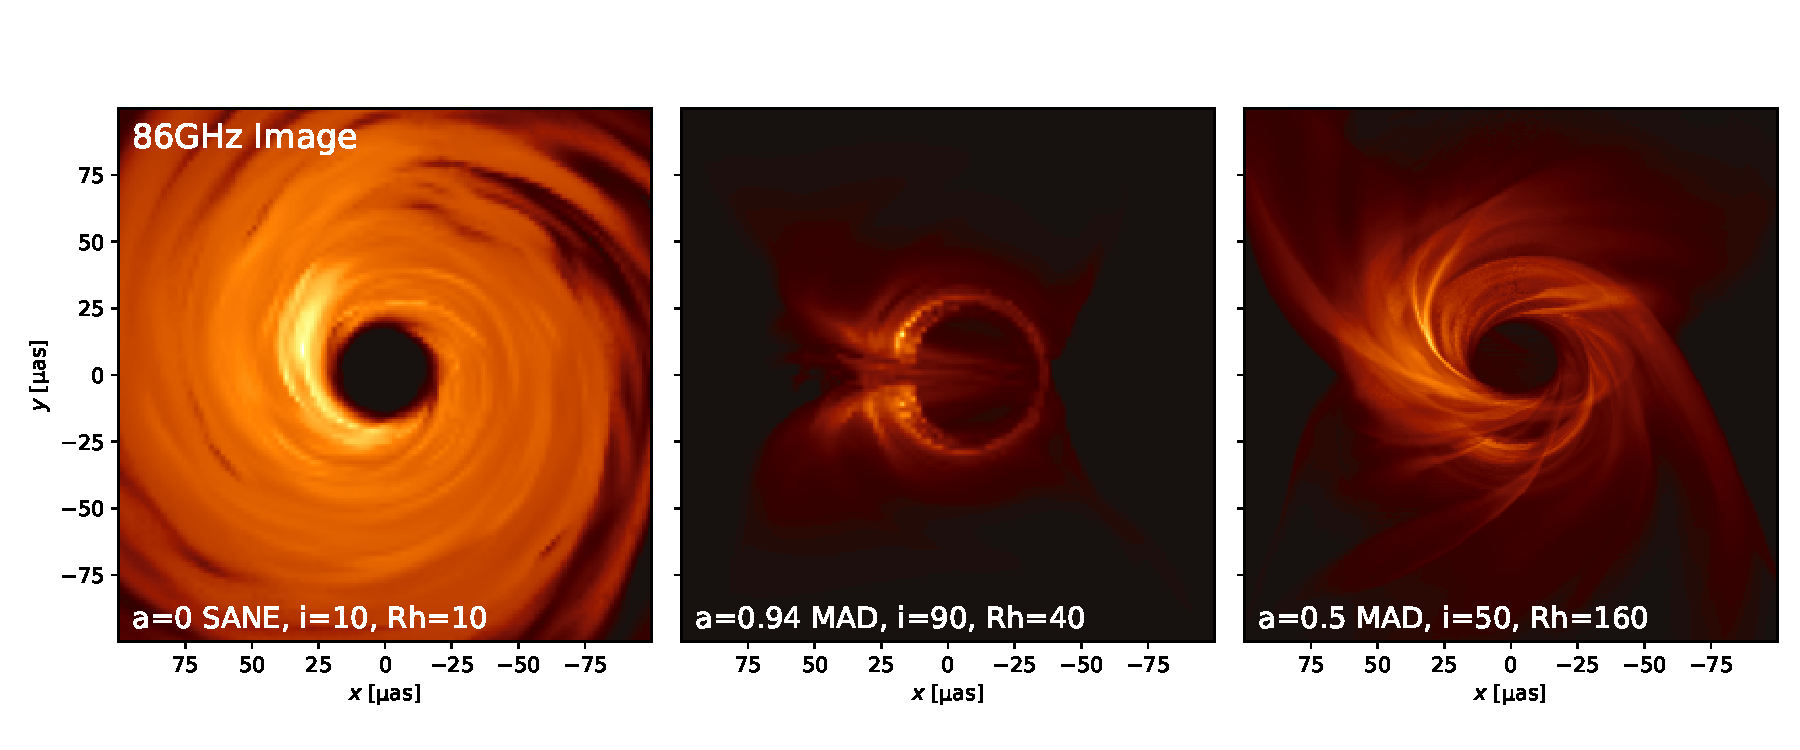
\includegraphics[width=\textwidth,trim=0 24 0 24]{figures/sample_86GHz.pdf}
  \caption{Sample 230\GHz and 86\GHz snapshot images from the simulation library:
    (\emph{left})~a thermal SANE,
    (\emph{middle})~a thermal MAD, and
    (\emph{right})~a non-thermal variable $\kappa$ MAD.
    Note that these models do not necessary pass any of the constraints.
    They simply demonstrate the variety of possible images.}
  \label{fig:sample_imgs}
\end{figure*}

%..............................................................................
\subsubsubsection{Electron Distribution Function}
\label{sec:eDF}

In \emph{thermal} models electron energies are distributed into the Maxwell-J{\"u}ttner distribution function:
\begin{align}
  \frac{1}{n_e}\frac{dn_e}{d\gamma} = \frac{\gamma^2 \sqrt{1-1/\gamma^2}} {\Theta_e K_2(1/\Theta_e)} \exp\left(-\frac{\gamma}{\Theta_e}\right);
\end{align}
recall $\Theta_e = k_b T_e/(m_e c^2)$, which is determined by the ion-electron temperature ratio $R \equiv T_i/T_e$:
\begin{align}
  T_e=\frac{2 m_p u}{3 k_B \rho (2+R)}.
\end{align}
Here $u$ and $\rho$ are the internal energy density and rest-mass density from the GRMHD simulation.
Thermal models are motivated by the idea that wave-particle scattering drives partial relaxation of the eDF, even though Coulomb scattering is ineffective.

Plasma heating models suggest that the partitioning of dissipation between ions and electrons depends on the local magnetic properties \citep[e.g.,][]{2010MNRAS.409L.104H, Kawazura771}.  This motivates a prescription in which the temperature ratio is a function of the plasma $\beta \equiv P_\mathrm{gas}/P_\mathrm{mag}$ \citep{2015ApJ...799....1C}.
We adopt the same model as \citetalias{M87PaperV} and \citetalias{M87PaperVIII}, where $R$ is a smooth function adopted from \cite{2016A&A...586A..38M}:
\begin{equation}
  R = \frac{T_i}{T_e} = \Rh \frac{b^2}{b^2+1} + \Rl \frac{1}{b^2+1}
  \label{eq:rhigh_prescription}
\end{equation}
where $b \equiv \beta/\beta_\mathrm{crit}$.
This model has three free parameters: $\beta_\mathrm{crit}$, $\Rl$, $\Rh$.  Here we take $\Rl = 1$ and $\beta_\mathrm{crit} = 1$, and allow $\Rh$ to vary from 1 to 160.

In \emph{non-thermal} models, the eDF has a power-law tail extending to high energy.
We explore two implementations in this paper:
\emph{i}) with a power-law distribution function
\begin{align}
  \frac{1}{n_e} \frac{d n_e}{d\gamma} &=
  \frac{p-1}{\gamma_{\min}^{1-p} - \gamma_{\vphantom{i}\max}^{1-p}}
  \gamma^{-p}
  \label{eq:nonthermaleDF}
\end{align}
which has power-law index $p$ and upper and lower limits $\gamma_{\min}$ and $\gamma_{\vphantom{i}\max}$; and
\emph{ii}) with a so-called $\kappa$ distribution function, inspired by observations of the solar wind and by results of collisionless plasma simulations \citep[e.g.,][and references therein]{2015JPlPh..81e3201K}
\begin{align}
  \frac{1}{n_e} \frac{d n_e}{d\gamma} =
  \gamma \sqrt{\gamma^2-1} \left(1+\frac{\gamma+1}{\kappa w}\right)^{-(\kappa+1)}
\end{align}
which has width parameter $w$ and power-law index parameter $\kappa$.

Evidently, any eDF assignment scheme is an approximation since the eDF depends in general on both local conditions and particle histories.  Notice that we also assume the eDF is isotropic, and neglect electron-positron pairs (see Section~\ref{sec:pair} for a discussion of potential impact of pair plasma for \sgra).

Once the eDF is specified, the radiative transfer coefficients (emissivities, absorptivities, and rotativities) can be readily calculated; see \cite{2021ApJ...921...17M} for a recent summary.

% cfg 11 dec: decided this is not essential.
%\kc{Perhaps add a plot of the different eDFs to display the variety of models considered.}

%..............................................................................
\subsubsubsection{Model Scaling}

With the exception of the special stellar wind-fed simulations, the GRMHD models considered in this work contain a characteristic speed, $c$, but are otherwise scale-free; they set $GM = c = 1$.
Physical scales are assigned during the radiative transfer step.
The black hole mass $\mbh$ fixes the length unit $\rg$ and time unit $\tg$.
Because the GRMHD models are not self-gravitating, one is free to set a density scale, or equivalently the accretion rate $\dot{M}$ or plasma mass scale $\Munit$ \citep[see, e.g.,][for a full discussion]{Wong_2022}.

% cfg, 11 dec 21: resolved this by reference to the PATOKA paper.  We really don't need all this anywhere else in the paper.
%The density in cgs units $\rho_\mathrm{cgs}$ is obtained from the density in simulation units $\rho_\mathrm{sim}$ via
%\begin{align}
%  \rho_\mathrm{cgs} = \rho_\mathrm{sim} \Munit_\mathrm{cgs} {(\rg)}_\mathrm{cgs}^{-3}.
%\end{align}
%Similarly, the energy density and magnetic fields in cgs units are set by:
%\begin{align}
%  u_\mathrm{cgs} &= u_\mathrm{sim} \Munit_\mathrm{cgs} {(\rg)}_\mathrm{cgs}^{-3} c_\mathrm{cgs}^2\\
%  B_\mathrm{cgs} &= (4\pi)^{1/2} B_\mathrm{sim} \Munit_\mathrm{cgs}^{1/2} (\rg)_\mathrm{cgs}^{-3/2} c_\mathrm{cgs};
%\end{align}
%the factor of $(4\pi)^{1/2}$ comes from converting Heaviside-Lorentz units (used in GRMHD simulations for efficiency) to cgs.
%\ckc{I found this notation confusion.  For example, $c$ is dimensional, although it's not necessary in cgs.  So I'm not sure what $c_\mathrm{cgs}$ really means here.  Is the dimensionless value of $c$ in cgs?  I'm probably too picky...}\monika{we just want to stress that c should be in cm/s}

The plasma mass scale parameter $\Munit$ controls the optical depth and thus the source brightness.  We adjust $\Munit$ iteratively until the time-averaged 230\GHz flux densities of the models are within a few percent of the $2.4\,\mathrm{Jy}$ mean observed during the 2017 campaign (see next section).  The reader should keep in mind that in this work model parameters are always varied at constant time-averaged millimeter flux density.

%Notice that the flux density is a nonlinear function of $\Munit$ because the accretion flow transits between the optical thick and thin regimes around 230\GHz.
%This makes the interpretations of the model trends in Section~\ref{sec:trends} less obvious.

%..............................................................................
\subsubsubsection{Radiative Transfer Calculation}


\begin{figure*}
  \centering
  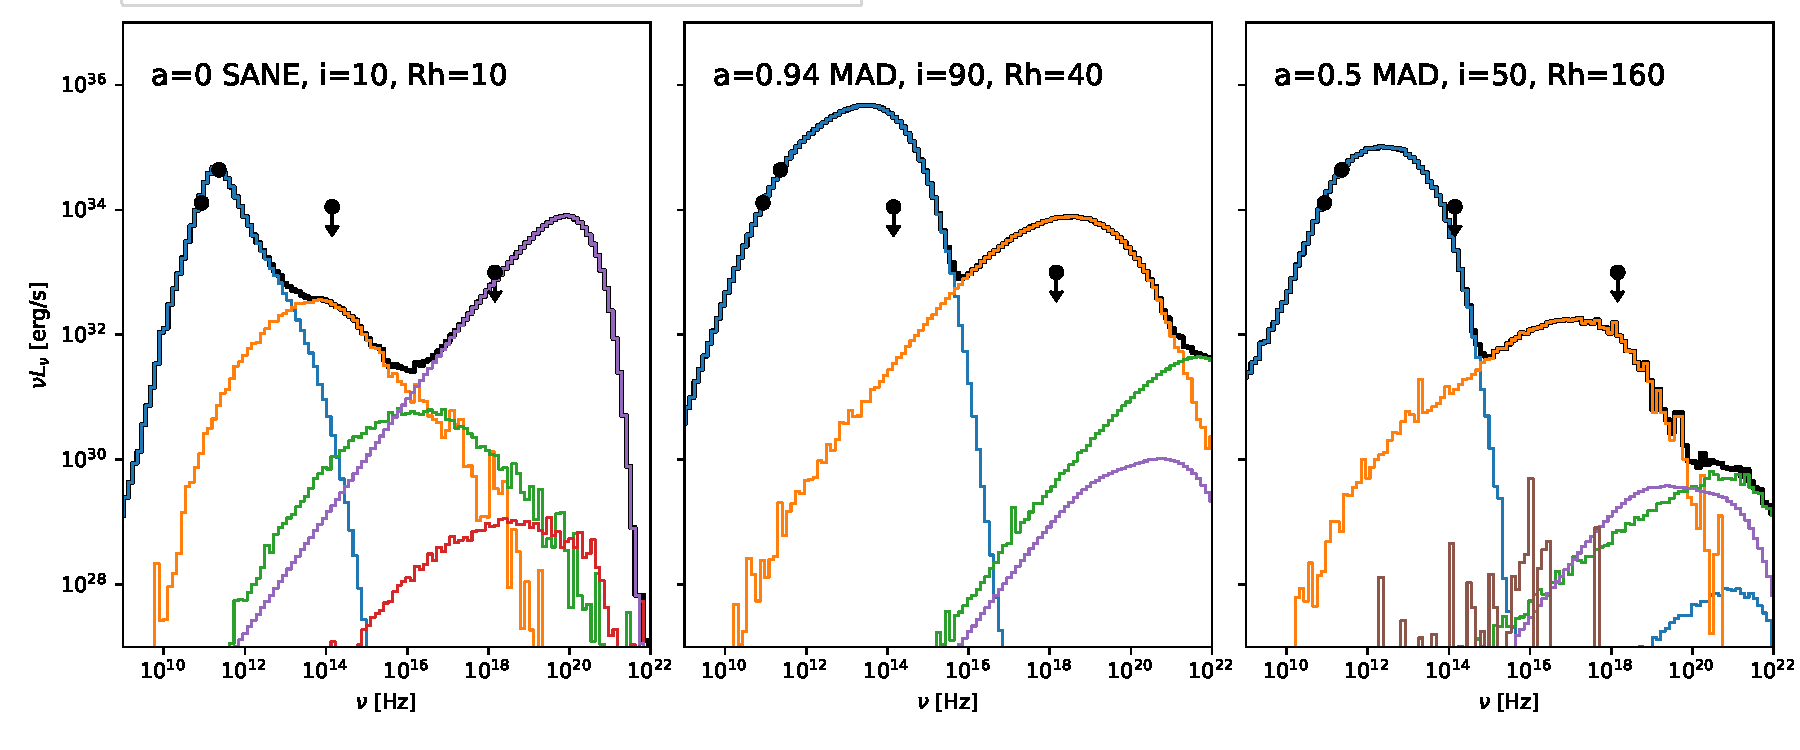
\includegraphics[width=\textwidth,trim=0 12 0 0]{figures/sample_sed.pdf}
  \caption{Sample SED from the simulation library:
    (\emph{left})~a thermal SANE,
    (\emph{middle})~a thermal MAD, and
    (\emph{right})~a non-thermal variable $\kappa$ MAD.
    Note that these models do not necessary pass any of the constraints.
    They simply demonstrate the variety of possible SEDs.
     %\ckc{That blocks the SED itself.  OK will try}
    }
  \label{fig:sample_SEDs}
\end{figure*}

Given an eDF, density scale $\Munit$, and radiative transfer coefficients, the emergent radiation is obtained by integrating the radiative transfer equation.
We use two classes of numerical methods: ray tracing to generate synthetic images, and Monte Carlo to generate spectral energy distributions (SEDs).
Further detail on numerical methods is given Appendix~\ref{app:radtrans}.
Comparisons of numerical methods \citep{2020ApJ...897..148G, Prather_et_al_2022} show that differences between radiative transfer schemes do not contribute significantly to the error budget.
% cfg 11 dec: done
%\ckc{Ben, please fill in paper title etc for the polarized radiative transfer comparison paper in refs.bib.}

The models are imaged at 86\GHz, 230\GHz\footnote{The mean frequency for  EHT observations is closer to 228\GHz.} and 2.2\um (near infrared, herafter NIR).
Direct imaging includes synchrotron and bremsstrahlung \citep[both ion-electron and electron-electron; see][for a recent review]{2020ApJ...898...50Y}.
The SED is averaged over a narrow range in inclination and over all azimuthal angles.
The SED includes synchrotron, bremsstrahlung, \emph{and} Compton scattering.
NIR emission is usually dominated by synchrotron, but we find that occasionally NIR synchrotron is so weak that Compton scattering overtakes.
The x-ray can be dominated by bremsstrahlung or Compton scattering, mainly depending on the electron temperature.
In Figures~\ref{fig:sample_imgs} and \ref{fig:sample_SEDs}, we present an illustrative set of model images and multiwavelength SEDs from our library.

All radiative transfer models used here set the emissivity to $0$ at $\sigma \equiv B^2/(8\pi\rho c^2) > \sigma_{cut} = 1$.  This is motivated by the notion that the numerical solution is unreliable at $\sigma > \sigma_{cut}$.  In particular numerical diffusion into the low density region (at the ``funnel wall'') makes the density too large, and truncation error in integration of the total energy equation produces large fractional errors in temperature.

%==============================================================================
\subsection{Summary of \sgra Model Library}

%You can check which data is available here:
%https://docs.google.com/spreadsheets/d/1gw9ichvvYGHLFsZl2wlxqu-O03qEULrwcw3Wixd8BhQ/edit#gid=930351969
%not sure that gives complete answer, but it will help.

A summary of all radiative transfer calculations is given in Table~\ref{tab:radiativemodels}. The entire image library
contains $6$ model sets; thousands of points in model parameter space and
%$364$ models (with different spins and electron prescriptions);
%$1,872,409 @230GHz and 86 GHz$
$\sim 1.8$M images in each of 86~GHz, 230~GHz, and $\sim0.5$M images in $2.2\mu$m;
%$1,233,100 SEDs$
$\sim1.2$M SEDs and occupies about $GGG$ gigabytes.

%\clearpage
%\pagebreak
%\movetabledown=3cm % recommended in AASTeX docs to center table on page
%\begin{rotatetable}
\begin{deluxetable*}{ccccccccccc}
\tabletypesize{\footnotesize}
\renewcommand{\arraystretch}{1.1}
\tablehead{
  \colhead{Model}              &%
  \colhead{$\Rl$}              &%
  \colhead{$\Rh$}              &%
  \colhead{$\beta_{\rm crit}$} &%
  \colhead{$p$}           &%
% \colhead{$\gamma_{\rm min/max}$} &%
  \colhead{$\kappa$}           &%
  \colhead{$i^\circ$}          &%
  \colhead{$\nu$}              &%
  \colhead{MWL SED}            &%
  \colhead{$\Delta t$}         &%
  \colhead{$\#frames$}     \\
  & & & & & & & \colhead{[GHz]} & & \colhead{[1000 M]} & [@230 GHz]}
\startdata
\multicolumn{11}{c}{\bf Thermal models}\\
\kharma & 1 & [1,10,40,160] & 1 & - & - & [10,30,...,170] & [86,230] & Yes & [15,20) & 360,000 \\
\kharma & 1 & [1,10,40,160] & 1 & - & - & [10,30,...,170] & [86,230] & Yes & [20-25) & 360,000 \\
\kharma & 1 & [1,10,40,160] & 1 & - & - & [10,30,...,170] & [86,230] & Yes & [25-30) & 360,000 \\
\bhac   & 1 & [1,10,40,160] & 1 & - & - & [10,30,...,90]  & [86,230] & No & [10-15) & 100,000 \\
\bhac   & 1 & [1,10,40,160] & 1 & - & - & [10,30,...,90]  & [86,230] & No & [20-25) & 100,000 \\
\bhac   & 1 & [1,10,40,160] & 1 & - & - & [10,30,...,90]  & [86,230] & No & [25-30) & 100,000 \\
\hamr   & 1 & [1,40,160]    & 1 & - & - & [10,50,90]      & [86,230] & Yes & [30-35) & 45,000 \\
\koral  & 1 & [20]          & 1 & - & - & [10,30,...,170] & [86,230] & No  & [5-100)   & 107,507 \\
Wind Accretion & 1 & [13,28]    & 1 & - & - & N/A        & [86,230] & No  & 10        & 1802 \\
\hamr Tilted    & 1 & [1,40,160] & 1 & - & - & [10,50,90] & [86,230] & Yes & [100-103) & 8,100 \\
\hline
\multicolumn{11}{c}{\bf Thermal + non-thermal power-law models} \\
\hamr & 1 & [1,40,160] & 1 & 4 & - & [10,50,90] & [86,230] & No & [30-35) & 45,000 \\
\hline
\multicolumn{11}{c}{\bf Thermal + non-thermal $\kappa$ models} \\
\bhac & 1 & [1,10,40,160]    & 1 & - & 3.5 ($\epsilon_0=0.05$) & [10,30,...,90]  & [86,230] & No & [25-30) & 20,000 \\
\bhac & 1 & [1,10,40,160]    & 1 & - & 3.5 ($\epsilon_0=0.10$) & [10,30,...,90]  & [86,230] & No & [25-30) & 20,000 \\
\bhac & 1 & [1,10,40,160]    & 1 & - & 3.5 ($\epsilon_0=0.20$) & [10,30,...,90]  & [86,230] & No & [25-30) & 20,000 \\
\bhac & 1 & [1,10,40,80,160] & 1 & - & variable $\kappa=\kappa(\beta,\sigma)$ & [10,30,...,90] & [86,230] & No  & [25-30) & 125,000 \\
\hamr & 1 & [1,10,40,160]    & 1 & - & variable $\kappa=\kappa(\beta,\sigma)$ & [10,30,...,90] & [86,230] & Yes & [30-35) & 100,000 \\
\enddata
\caption{Summary of emission simulations in \sgra EHT model library. In case of the Wind Accretion the viewing angle is set by the boundary conditions used in the model and the $\rhigh$ parameter is constrained by the observed 230\,GHz flux (the two reported values correspond to two models with different magnetizations).
%\monika{why is wind model inclination N/A? can anyone explain?}
%\gw{I didn't write N/A, but as I recall from Sean, the wind models *have* an absolute orientation with respect to Earth because of how their boundary condition is set up, so it wouldn't make sense to vary inclination. Also their bhspin = 0.}\monika{Ah, ok , so there is an inclination but we dont know it. can you find out ? maybe I can also change the Fig 1 accordingly (although that would require some thinking)!}\gw{sorry not sure what you mean by ``there is an inclination''. there is an inclination that we plug into ipole, but that inclination is with respect to the coordinate system, not anything particularly ``physical'' (because the black hole has zero spin). the coordinate system is oriented such that images are computed at inc->180 (inc as defined in the ipole sense)}\monika{ok, this makes no sense since from our point of view the "boundary conditions" for this model are fixed...we should just find best rhigh for our viewing angle..}
%The cadence of KHARMA=5M, BHAC=10M for thermal and nonthermal variable kappa, 50M for nonthermal variable efficiency models, and HAMR=10M for thermal, nonthermal powerlaw and variable kappa.
%\gw{Rhigh for the wind accretion models is either 28 or 13, but these are for two separate simulations (so it's not like there's one simulation where Rhigh has been varied); no SED from grmonty-like codes, but there is ``SED''-like information from imaging at different frequencies}\monika{how many 230 ghz frames we have for these two wind models and within what times??}
}~\label{tab:radiativemodels}
\end{deluxetable*}
%\end{rotatetable}

%\pagebreak
%\clearpage
% %..............................................................................
% \subsubsection{Thermal Models}
%
% ...
%
% \paragraph{Illinois Models}
%
% % Please fill in basic information of the models in the following list.
% % Please add more details if necessary. A full paragraph description
% % of the model is welcome, but not required at this point.
% \begin{itemize}[noitemsep]
% \item $a_\mathrm{spin}$: 0, $\pm1/2$, $\pm15/16$
% \item Magnetic Flux: MAD, SANE
% \item Adiabatic Index $\Gamma$: 4/3
% \item Time $t_\mathrm{final}$: 30,000$M$
% \item $\rho_0$: 3 different density normalization chosen for each parameter set for $t \in [15,000, 20,000), [20,000, 25,000), [25,000, 30,000)$.
% \item $\Rh$: 1, 10, 40, 160
% \item Inclination $i$: 10$^\circ$, 30$^\circ$, 50$^\circ$, ..., 170$^\circ$
% \item Resolution:
% \item Initial conditions:
% \item Reference: this work
% \item Status: w4 and w5 all done; w3 in progress
% \end{itemize}
%
% \paragraph{Frankfurt Models}
%
% % Please fill in basic information of the models in the following list.
% % Please add more details if necessary. A full paragraph description
% % of the model is welcome, but not required at this point.
% \begin{itemize}[noitemsep]
% \item $a_\mathrm{spin}$: 0, $\pm1/2$, $\pm15/16$
% \item Magnetic Flux: MAD, SANE
% \item Adiabatic Index $\Gamma$: 4/3
% \item Time $t_\mathrm{final}$: 30000
% \item $\rho_0$: 3 different density normalizations chosen for each parameter set for $t \in [10,000, 15,000), [20,000, 25,000), [25,000, 30,000)$
% \item $\Rh$: 1, 2.5, 5, 10, 40, 160
% \item Inclination $i$: 10$^\circ$, 30$^\circ$, 50$^\circ$,..., 90$^\circ$
% \item Resolution:
% \item Initial conditions:
% \item Reference: this work
% \item Status: all done except for SANE a=-15o16
% \end{itemize}
%
% \paragraph{HAMR Models}
%
% % Please fill in basic information of the models in the following list.
% % Please add more details if necessary. A full paragraph description
% % of the model is welcome, but not required at this point.
% \begin{itemize}[noitemsep]
% \item $a_\mathrm{spin}$: 0, $\pm1/2$, $\pm15/16$
% \item Magnetic Flux: MAD, SANE
% \item Adiabatic Index $\Gamma$: 13/9, 5/3
% \item Time $t_\mathrm{final}$: $35,000M$
% \item $\rho_0$: 1 density normalization for $[30,000-35,000)M$
% \item $\Rh$: 1, 40, 160
% \item Inclination $i$: 10$^\circ$, 50$^\circ$, 90$^\circ$
% \item Resolution: $348\times 192\times 192$, $240\times 192\times 192$
% \item Initial conditions: FM: $r_{\rm in}=6, 20M$; $r_{\rm pmax}=12, 41M$
% \item Grid outer radius: $1000M$, $200M$
% \item Reference: this work
% \item Status: GRMHD simulations done
% \end{itemize}
%
% %..............................................................................
% \subsubsection{Non-thermal (power-law )Models}
%
% ...
%
% \paragraph{Frankfurt Models}
%
% % Please fill in basic information of the models in the following list.
% % Please add more details if necessary. A full paragraph description
% % of the model is welcome, but not required at this point.
% \begin{itemize}[noitemsep]
% \item $a_\mathrm{spin}$: 0, $\pm1/2$, $\pm15/16$
% \item Magnetic Flux: MAD, SANE
% \item Adiabatic Index $\Gamma$:
% \item Time $t_\mathrm{final}$:
% \item $\rho_0$:
% \item Power law fraction $f$:
% \item Power law index $p$:
% \item Inclination $i$:
% \item Reference:
% \item Status: no power-law model so far
% \end{itemize}

% \paragraph{HAMR Models}

% % Please fill in basic information of the models in the following list.
% % Please add more details if necessary. A full paragraph description
% % of the model is welcome, but not required at this point.
% \begin{itemize}[noitemsep]
% \item $a_\mathrm{spin}$: 0, $\pm1/2$, $\pm15/16$
% \item Magnetic Flux: MAD, SANE
% \item Adiabatic Index $\Gamma$: 13/9, 5/3
% \item Time $t_\mathrm{final}$: $35,000M$
% \item $\rho_0$: 1 density normalization for $[30,000-35,000)M$
% \item $\Rh$: 1, 40, 160
% \item Inclination $i$: 10$^\circ$, 50$^\circ$, 90$^\circ$
% \item Resolution: $348\times 192\times 192$, $240\times 192\times 192$
% \item Initial conditions: FM: $r_{\rm in}=6, 20M$; $r_{\rm pmax}=12, 41M$
% \item Grid outer radius: $1000M$, $200M$
% \item Reference: this work
% \item Status: GRMHD simulations same as for thermal models
% \end{itemize}
%
% %..............................................................................
% \subsubsection{Non-thermal ($\kappa$) Models}
%
% ...
%
% % Please fill in basic information of the models in the following list.
% % Please add more details if necessary. A full paragraph description
% % of the model is welcome, but not required at this point.
% \begin{itemize}[noitemsep]
% \item $a_\mathrm{spin}$: 0, $\pm1/2$, $\pm15/16$
% \item Magnetic Flux: MAD, SANE
% \item Adiabatic Index $\Gamma$:
% \item Time $t_\mathrm{final}$:
% \item $\rho_0$:
% \item $\kappa$:
% \item Inclination $i$:
% \item Reference:
% \item Status:
% \end{itemize}
%
% \paragraph{Frankfurt Models}
%
% % Please fill in basic information of the models in the following list.
% % Please add more details if necessary. A full paragraph description
% % of the model is welcome, but not required at this point.
% \begin{itemize}[noitemsep]
% \item $a_\mathrm{spin}$: 0, $\pm1/2$, $\pm15/16$
% \item Magnetic Flux: MAD, SANE
% \item Adiabatic Index $\Gamma$: 4/3
% \item Time $t_\mathrm{final}$: 30000
% \item $\rho_0$: individual normalisation for each kappa model; only  for $t \in [25,000, 30,000)$
% \item $\kappa$: variable $\kappa(\beta, \sigma)$, fixed $\kappa=3.5$ with $\epsilon=\epsilon_{0} f(\beta,\sigma)$ for $\epsilon_{0}=0.05,0.10,0.20$
% \item $\Rh$: 1, 2.5, 5, 10, 40, 160
% \item Inclination $i$: 10$^\circ$, 30$^\circ$, 50$^\circ$,..., 90$^\circ$
% \item Reference: this work
% \item Status: in production
% \end{itemize}
%
% \paragraph{HAMR Models}
%
% % Please fill in basic information of the models in the following list.
% % Please add more details if necessary. A full paragraph description
% % of the model is welcome, but not required at this point.
% \begin{itemize}[noitemsep]
% \item $a_\mathrm{spin}$: 0, $\pm1/2$, $\pm15/16$
% \item Magnetic Flux: MAD, SANE
% \item Adiabatic Index $\Gamma$: 13/9, 5/3
% \item Time $t_\mathrm{final}$: $35,000M$
% \item $\rho_0$: 1 density normalization for $[30,000-35,000)M$
% \item $\kappa$: variable $\kappa (\beta, \sigma)$
% \item $\Rh$: 1, 40, 160
% \item Inclination $i$: 10$^\circ$, 50$^\circ$, 90$^\circ$
% \item Resolution: $348\times 192\times 192$, $240\times 192\times 192$
% \item Initial conditions: FM: $r_{\rm in}=6, 20M$; $r_{\rm pmax}=12, 41M$
% \item Grid outer radius: $1000M$, $200M$
% \item Reference: this work
% \item Status:
% \end{itemize}
%
% %..............................................................................
% \subsubsection{Critical $\beta$ Models}
%
% % Please fill in basic information of the models in the following list.
% % Please add more details if necessary. A full paragraph description
% % of the model is welcome, but not required at this point.
% \begin{itemize}[noitemsep]
% \item $a_\mathrm{spin}$:
% \item Magnetic Flux: MAD, SANE
% \item Adiabatic Index $\Gamma$:
% \item Time $t_\mathrm{final}$:
% \item $\rho_0$:
% \item Power law fraction $f$:
% \item Power law index $p$:
% \item Inclination $i$:
% \item Reference:
% \item Status:
% \end{itemize}
%
% %..............................................................................
% \subsubsection{Stellar Wind Accretion Models}
%
% % Please fill in basic information of the models in the following list.
% % Please add more details if necessary. A full paragraph description
% % of the model is welcome, but not required at this point.
% \begin{itemize}[noitemsep]
% \item $a_\mathrm{spin}$: 0
% \item Magnetic Flux: MAD, SANE
% \item Adiabatic Index $\Gamma$:
% \item Time $t_\mathrm{final}$:
% \item $\rho_0$:
% \item Power law fraction $f$:
% \item Power law index $p$:
% \item Inclination $i$:
% \item Reference:
% \item Status:
% \end{itemize}
%
% %..............................................................................
% \subsubsection{Koral Long MAD Models}
%
% % Please fill in basic information of the models in the following list.
% % Please add more details if necessary. A full paragraph description
% % of the model is welcome, but not required at this point.
% \begin{itemize}[noitemsep]
% \item $a_\mathrm{spin}$: 0, $\pm0.3$, $\pm0.5$, $\pm0.7$, $\pm0.9$
% \item Magnetic Flux: MAD
% \item Adiabatic Index $\Gamma$:
% \item Time $t_\mathrm{final}$: 100,000$M$
% \item $\rho_0$:
% \item Power law fraction $f$:
% \item Power law index $p$:
% \item Inclination $i$:
% \item Reference:
% \item Status:
% \end{itemize}
%
% %..............................................................................
% \subsubsection{Tilted Models}
%
% % Please fill in basic information of the models in the following list.
% % Please add more details if necessary. A full paragraph description
% % of the model is welcome, but not required at this point.
% \begin{itemize}[noitemsep]
% \item $a_\mathrm{spin}$: $+15/16$
% \item Magnetic Flux: INSANE
% \item Adiabatic Index $\Gamma$: 5/3
% \item Time $t_\mathrm{final}$: $>100,000M$
% \item $\rho_0$: 1 density normalization for $[100,000-103,000)M$
% \item $\Rh$: 1, 40, 160
% \item Inclination $i$: 10$^\circ$, 50$^\circ$, 90$^\circ$
% \item Resolution: $448\times 144\times 240$,
% \item Initial conditions: FM: $r_{\rm in}=12.5M$; $r_{\rm pmax}=25M$
% \item Grid outer radius: $100,000M$
% \item Reference: Chatterjee+20, Liska+18
% \end{itemize}
